%!TEX root = iclr2026_conference.tex
% 2026-09-25 PROSE PASS (owner directive): claim-first rewrites and token glosses in A/H/K prose; numeric dumps already tabulated in tab:app:coverage/frontier/secondparam/repro deduplicated to table pointers. No number, status, citation, label or claim changed; every removed value remains in its table.
% Binds outline appendix content classes — manuscript/writing_outline_boundary_paper.md (v2.0);
% ==== BRIEF APP (\appendix) ===============================================
% [中] 定位：附录是这项测量的仪器档案；正文的数字在此找到各自的协议、覆盖账目与产物来源。
% 主张：附录给出正文结论所依赖的机制、账目与 inventory 记录，不放宽正文任何范围。
% 证据：冻结计划、typed failure 账本、coverage 表、checkpoint 清单、各附录声明的 inventory。
% 手法/边界：Li 式把数据当仪器，He 式平铺；不是第二个结果节，附录数字不扩大正文范围。
% [EN] Role: the instrument record behind the main-text numbers.
% Claim: the appendix holds the mechanics and accounts behind the main claims.
% Evidence: frozen plans, typed-failure ledgers, coverage tables, checkpoint inventories,
% declared inventories.
% Craft/Boundaries: data as instrument, stated flat; not a second results section; no appendix
% number widens a main-text scope.
% ==== /BRIEF ==============================================================
\appendix


\section{Use of LLM Statement}
\label{app:llm-usage}

An LLM was used only for polishing language; the scientific content is entirely original.


% ==== BRIEF APP A (sec:app:protocol) ======================================
% [中] 定位：先定规则再看结果；后文每一节都用这里定义的生命周期、disposition 词表与测量约定。
% 主张：每个产物都在冻结计划下产生，每个执行的问题都以三个逐字 token 之一收尾。
% 证据：五阶段生命周期、plan.json、#77 发布布局、三个 disposition token、per-ticket 预算。
% 手法/边界：He 式定义句，名词先行；这是约定，不是结果，不得读作任何问题的答案。
% [EN] Role: rules before results; every later section uses the conventions defined here.
% Claim: every artifact comes from a frozen plan; every question ends in one token.
% Evidence: the five-stage lifecycle, plan.json, the #77 publication layout, the three
% disposition tokens.
% Craft/Boundaries: definitions, nouns first; conventions, not findings; never read as the
% answer to any question.
% ==== /BRIEF ==============================================================
\section{Protocol Mechanics and Measurement Conventions}
\label{sec:app:protocol}

% ==== BRIEF APP A ¶1 (lifecycle) ==========================================
% [中] 定位：交代冻结计划的生命周期；"结果不回流到计划"这一保证由此而来。
% 主张：计划在任何结果之前以实际数值冻结；任何源码改动之后 runner 拒绝执行。
% 证据：五阶段；plan.json 固定 membership、seed、estimand、disposition 规则；--validate 须 exit 0。
% 手法/边界：按阶段一句一事；保留"被取代的旧计划从未用于任何结果"；是保证，不是结果证据。
% [EN] Role: the frozen-plan lifecycle; no outcome feeds back into a plan.
% Claim: plans freeze with actual values before any outcome; source edits block execution.
% Evidence: freeze, validate, execute, publish, exact-validate; plan.json pins membership,
% seeds, and disposition rules; --validate recomputes every published table and must exit 0.
% Craft/Boundaries: stages in order, one fact each; keep "superseded plans fed no outcome"; a
% guarantee, not a result.
% ==== /BRIEF ==============================================================
% VOCAB-PASS: Explain disposition as a rule-assigned outcome category.
This section defines the protocol lifecycle and the measurement conventions that every downstream section uses. Throughout the appendices, $h$ denotes the requested horizon $\Delta$ of Section~\ref{sec:mth:setting}, counted in carrier frames.
Every executed artifact in this paper is produced under a frozen plan. The lifecycle has five stages: freeze, validate, execute, publish, exact-validate. At the freeze stage the runner writes \texttt{plan.json}, which pins membership, templates, seeds, estimands, metrics, contrasts, compute accounting, and stop rules; a freeze contains actual numerical values, and approximations or example values in place of values are banned. After the freeze, loading the plan re-hashes the source tree and the runner refuses to execute after any source edit. The validate stage checks the plan before any outcome is computed, execution then runs every scheduled cell, and publication writes the \#77 layout (\texttt{summary.json}, \texttt{comparisons.csv}, \texttt{findings.md}) beside the producing module. The exact-validate stage reruns a \texttt{-{}-validate} mode that recomputes every published table from the artifacts and must exit 0. Campaign runners additionally write \texttt{inventory.json}, \texttt{campaign.json}, \texttt{ledger.json}, \texttt{coverage.json}, per-branch \texttt{markers/}, \texttt{receipts/}, and \texttt{attempts/}, and their \texttt{-{}-validate} mode re-derives \texttt{coverage.json} from the retained ledger. A recorded reseal guard regenerates a plan through its own prepare module and aborts unless the only drift is recorded source text, with membership, branches, and prior-exposure byte-identical. Superseded pre-review plans stay on disk and were never used for any outcome.

% ==== BRIEF APP A ¶2 (typed failures) =====================================
% [中] 定位：定义 typed failure；后文所有覆盖数与 per-state 候选数都按此约定计。
% 主张：每个排定 cell 要么执行，要么作为 typed terminal failure 保留；无按结果的排除、重试、替换。
% 证据：native-manifest 超时、paired-view 不匹配、prior_candidate_absent、compute_allowance_exceeded。
% 手法/边界：禁止项用平铺否定句列出；未资助 cell 记 unsupported；失败不得读作被丢弃或按最差计。
% [EN] Role: defines the typed failure; later coverage and candidate counts use it.
% Claim: each scheduled cell runs or stays as a typed terminal failure.
% Evidence: native-manifest deadlines, paired-view mismatches, prior_candidate_absent,
% compute_allowance_exceeded; per-ticket allowances of four and six GPU-hours.
% Craft/Boundaries: no outcome-conditioned exclusion, retry, replacement, or re-freeze;
% unfunded cells are recorded unsupported, never dropped.
% ==== /BRIEF ==============================================================
% VOCAB-PASS: Define typed terminal failures before listing failure kinds.
A typed terminal failure is a scheduled cell retained with its failure kind when it cannot complete. Every scheduled cell is executed or retained as a typed terminal failure. There is no outcome-conditioned exclusion, retry, replacement, or re-freeze. A terminal-incomplete ledger refuses top-up permanently, and all failure records are kept. Allowances were recorded per ticket, and an unfunded cell is recorded \texttt{unsupported}, never dropped.

% ==== BRIEF APP A ¶3 (disposition tokens) =================================
% [中] 定位：固定全文判定用语；每个执行的问题只落在三个逐字 token 之一。
% 主张：词表恰有三个 token，均由结果之前声明的规则给出，唯一例外已披露。
% 证据：Section 4 restatement 在 oracle-pass 与 completion-pass 结果之后指定；C19 重读标 post hoc。
% 手法/边界：token 一字不改；例外与规则同段写明；不得软化为等价或"无显著差异"。
% [EN] Role: fixes the verdict vocabulary; one verbatim token per executed question.
% Claim: three tokens, each from a rule declared before outcomes, one exception disclosed.
% Evidence: supported, not_supported_by_this_experiment, readiness_or_precision_insufficient;
% one positive and one indeterminate port gave the third; the C19 re-readings are post hoc.
% Craft/Boundaries: tokens verbatim; the exception beside the rule; never softened into
% equivalence language.
% ==== /BRIEF ==============================================================


% ==== BRIEF APP A ¶4 (measurement discipline) =============================
% [中] 定位：统一测量约定；后文每个区间、estimand 与 13-candidate 计数都按此读。
% 主张：配对 bootstrap 区间只作描述，不作显著性检验，不做多重校正；zero-shot 与 few-shot 不合并。
% 证据：对右删失 t=600 窗末 replay cost 的 normalized regret；冻结 13 候选 a00 + a01--a12。
% 手法/边界：区间不是检验；proxy cost 不是已定成本；13 候选只限 N1 closed-loop 与 proxy-era 记录。
% [EN] Role: one measurement convention; every later interval and estimand reads through it.
% Claim: intervals are descriptive, never tests; zero-shot and few-shot are never pooled.
% Evidence: no multiplicity adjustment; regret against the right-censored t=600 replay cost;
% the frozen 13-candidate set a00 plus a01--a12; 16, 11, 20 declared elsewhere.
% Craft/Boundaries: no interval-as-test; the proxy is not a settled cost; 13 candidates bind to
% N1 closed-loop and proxy-era records.
% ==== /BRIEF ==============================================================
Measurement discipline is uniform. All paired contrasts carry bootstrap intervals over paired units, labelled descriptive, and no interval is read as a significance test. No multiplicity adjustment is applied. Zero-shot and few-shot conditions are reported separately and never pooled. Evaluation states are held-out lineages with at least one coverage-admissible branch, taken in sorted identity order. In the N1 record the candidate inventory is the frozen 13-candidate set (reference \texttt{a00} plus angular candidates \texttt{a01}--\texttt{a12}), with per-state counts reduced by typed branch failures.

% ==== BRIEF APP A ¶5 (compute accounting) =================================
% [中] 定位：交代算力账目；后文每个跨系统对比都附这份工作量前沿。
% 主张：更新数相同，但训练与推理都不是算力匹配；报告的是工作前沿，不是等量化。
% 证据：9,000 次更新、batch 64、576,000 样本；training_compute_matched=false；1,862,396 对 1,837,690。
% 手法/边界：先说不是什么再说是什么；候选数、参数数、2% 宽度容差都不是算力匹配。
% [EN] Role: the compute accounting behind every cross-system contrast.
% Claim: updates are equalized; training and inference are not compute-matched.
% Evidence: 9,000 updates at batch 64, 576,000 examples; training_compute_matched=false; #74
% fits of 1,862,396 versus 1,837,690 parameters, relative difference 0.0134.
% Craft/Boundaries: what it is not, then what it is; active capacity is not claimed equal.
% ==== /BRIEF ==============================================================
Compute accounting reports per-state wall time, active-parameter step counts, and candidate counts. Training is equalized: 9{,}000 updates with batch 64 per cell, which is 576{,}000 examples, and identical minibatches per paired seed across arms. Linear MACs are reported rather than full FLOPs. The capacity contract matches the continuous width to the hybrid total parameter count within a 2\% tolerance; the \#74 fits measure 1{,}862{,}396 continuous versus 1{,}837{,}690 hybrid parameters, a relative difference of 0.0134. All fits ran on one RTX 3090 under an exclusive lock, and every port targets the existing $\sim$1.8M-parameter frozen-carrier predictor scale. All fits ran on one RTX 3090 under an exclusive lock, and every port targets the existing $\sim$1.8M-parameter frozen-carrier predictor scale.

% ==== BRIEF APP A ¶6 (seeds) ==============================================
% [中] 定位：固定种子账；复现与 seed 区间不交叠都依赖这里。
% 主张：配对 checkpoint 在四个再训练族上共用三个 seed；campaign 与 engine seed 与此前区间不交叠。
% 证据：20260908、20260909、20260910；#77 基数 764,000,000+ordinal 与 764,100,000+ordinal。
% 手法/边界：纯记账段，数字照抄；三个 seed 给出配对 checkpoint，不是推断性结论的样本。
% [EN] Role: pins the seed ledger that reproduction depends on.
% Claim: three seeds shared by four retraining families; campaign and engine seeds disjoint.
% Evidence: 20260908, 20260909, 20260910; #77 bases 764,000,000+ordinal and
% 764,100,000+ordinal; 764,200,000+ to 764,400,000+ reserved.
% Craft/Boundaries: a ledger, numbers copied exactly; three seeds pair checkpoints, not an
% inferential sample.
% ==== /BRIEF ==============================================================
Paired checkpoints use three seeds, 20260908, 20260909, and 20260910, across the retraining families. Campaign generation and engine seeds are pinned disjoint from all earlier ranges in each frozen plan. The \#77 bases are 764{,}000{,}000+ordinal for generation and 764{,}100{,}000+ordinal for the engine, with 764{,}200{,}000+, 764{,}300{,}000+, and 764{,}400{,}000+ reserved for the \#75-adjacent N2 capture, engine, and adaptation streams. Table~\ref{tab:app:checkpoints} inventories the per-seed artifacts.

% #91-WP5: full protocol element list moved from method.tex (was §4 ¶2).
% ==== BRIEF APP A ¶7 (protocol element list) ==============================
% [中] 定位：正文 §4 只点名协议纪律；这里给出移自正文的完整定义，供引用时核对。
% 主张：协议由四条设计纪律与五条计分报告纪律构成，每条在此完整定义。
% 证据：208/208 已尝试；novel 侧 186/208；normal 侧 34/104，70 个 typed failure 保留；480 个 CLEVRER 窗口。
% 手法/边界：粗体名 + 括号定义逐条平铺；95% 区间不支持优越性判定；负结果不改写为"no significant difference"。
% [EN] Role: the full protocol list; the main text names each discipline, this defines it.
% Claim: four design disciplines and five scoring-and-reporting disciplines.
% Evidence: 208/208 normal-mechanics branches attempted; 186/208 admissible novel side; 34/104
% normal side, all 70 contention-era failures kept; 480 CLEVRER windows, zero typed failures.
% Craft/Boundaries: bold name, parenthetical definition; the 95% intervals support no
% superiority decision.
% ==== /BRIEF ==============================================================
The protocol's design discipline is \textbf{frozen plans} (every campaign, training run, and evaluation run executes a plan frozen before launch and re-hashed at launch, refusing the run after any source edit); \textbf{sealed membership} (cell membership, held-out state identities, and the candidate inventory are pinned before any rendered run or model score, and no outcome moves membership); \textbf{typed terminal failures} (every scheduled unit ends admissible or as a typed failure with a recorded kind, retained and reported per cell, never silently dropped or worst-cased); and \textbf{equal-update training with work reporting} (paired arms share minibatches and update budgets, and the continuous width is matched to the hybrid parameter count within a width tolerance). Its scoring discipline is \textbf{paired descriptive inference} (contrasts report mean paired differences over paired units with descriptive 95\% paired-bootstrap intervals); a \textbf{declared candidate inventory} (the 13 candidate actions per state, one reference drag plus 12 release-angle actions, are pinned before scoring, typed branch failures remove candidates without refill, and CLEVRER runs no inventory); and \textbf{every attempted cell reported} (the accounting is fixed in advance and reported in full, with all typed failures retained).


% ==== BRIEF Table (tab:app:checkpoints) ===================================
% [中] 定位：checkpoint 的物理清单；每个被评估的模型都能追到磁盘上的具体文件。
% 主张：四个再训练族的每个 seed 都有可定位的 checkpoint，且按相同更新预算训练。
% 证据：#74、#77、#79 各六个 fit、9,000 次更新；#78 六个 tawm/vlwm fit，continuous 参照为冻结 #77、不重训。
% 手法/边界：caption 只说清单与配对 seed；不是性能表，也不是算力匹配。
% [EN] Role: the physical checkpoint inventory; every model traces to a file.
% Claim: every seed of four retraining families has a locatable checkpoint.
% Evidence: #74, #77, #79 six fits each; #78 six tawm and vlwm fits at the identical budget,
% with frozen #77 continuous references not retrained.
% Craft/Boundaries: inventory and paired seeds only; not a performance table, not compute
% matching.
% ==== /BRIEF ==============================================================
\begin{table}[t]
\centering
\small
\caption{Per-seed checkpoint inventory. All rows use paired seeds 20260908, 20260909, and 20260910 with identical minibatches per paired seed.}
\label{tab:app:checkpoints}
\begin{tabular}{@{}p{0.30\textwidth}p{0.17\textwidth}p{0.40\textwidth}@{}}
\toprule
Family and root & Arms & Per-seed artifacts and budget \\
\midrule
\#74 matched systems, \texttt{.local-artifacts/}\newline\texttt{issue-\allowbreak 74-\allowbreak matched-\allowbreak dynamics-\allowbreak v1} & \texttt{continuous}, \texttt{hybrid} & \texttt{seed-\allowbreak */\allowbreak \{continuous,hybrid\}/}\newline\texttt{\{predictor,controller\}.pt}; six fits, 9{,}000 updates each, selection at the last update \\
\#77 N1 retraining, \texttt{.local-artifacts/}\newline\texttt{issue-77-n1-dynamics-v1} & \texttt{continuous}, \texttt{hybrid} & \texttt{seed-\allowbreak */\allowbreak \{continuous,hybrid\}/}; six fits, 9{,}000 updates each, identical recipe to \#74 \\
\#79 CLEVRER replication, \texttt{.local-artifacts/}\newline\texttt{issue-\allowbreak 79-\allowbreak clevrer-\allowbreak boundary-\allowbreak v1} & \texttt{continuous}, \texttt{hybrid} & \texttt{seed-\allowbreak */\allowbreak \{continuous,hybrid\}/}\newline\texttt{predictor.pt}; six fits, 9{,}000 updates each \\
\bottomrule
\end{tabular}
\end{table}

\section{CLEVRER Replication Details}
\label{sec:app:clevrer}

% ==== BRIEF APP clevrer ¶1 data provenance ================================
% [中] 定位：数据出处与字段契约；下游每个带掩码的估计量都依赖此处的 inside_camera_view。
% 主张：只用官方注释档案，不下载视频，也不重新生成场景。
% 证据：train 156,761,889 字节（e7f9185a），val 78,386,966 字节（d89e7471）；98b8420 仅模型代码。
% 手法/边界：约定非结果；字段不足即发 readiness_or_precision_insufficient 是反事实规则，未触发。
% [EN] Role: data provenance and the field contract every masked estimand uses.
% Claim: only the official annotation archives were used: no videos, no regenerated scenes.
% Evidence: 156,761,889 and 78,386,966 bytes (e7f9185a, d89e7471); 98b8420 is model code.
% Craft/Boundaries: a convention; the readiness_or_precision_insufficient rule never fired.
% ==== /BRIEF ==============================================================
This section documents the CLEVRER replication: data provenance, frozen membership rule, Phase-0 vocabulary mapping, endpoint grid, and training protocol.
The data source is the official CLEVRER release at \texttt{data.csail.mit.edu/\allowbreak clevrer} under a CC0 license \citep{yi2020clevrer}. Only the annotation archives were used: train at 156{,}761{,}889 bytes with \texttt{sha256} prefix \texttt{e7f9185a} and validation at 78{,}386{,}966 bytes with prefix \texttt{d89e7471}. No videos were downloaded. Train scenes 0--9999 and validation scenes 10000--14999 ship annotations, and the test split ships none. Each annotation contains \texttt{object\_property} records for color, material, and shape, per-frame \texttt{motion\_trajectory} entries with per-object location, orientation, velocity, and angular velocity, collision events with \texttt{frame\_id}, and an \texttt{inside\_camera\_view} flag. That flag is the availability mask, applied in slot columns 7 and 10 and in every masked estimand, and unavailable fields are zeroed exactly as the deployment carrier zeroes them. Vertical location and velocity, orientation matrices, and angular velocities are parsed into per-scene shards for the parser-contract record with no carrier-column referent. No official generation or simulation code exists. The public CLEVRER repository at pinned commit \texttt{98b8420} contains model code only, and the paper's Bullet-plus-Blender pipeline was never released, so regenerated scenes are not a fallback. Had the released fields proved insufficient for the feature-parser contract, the frozen rule required publishing \texttt{readiness\_or\_precision\_\allowbreak insufficient} naming the exact blocker.

% ==== BRIEF APP clevrer ¶2 frozen membership ==============================
% [中] 定位：成员规则；它保证 12 个场景不是按结果挑出来的。
% 主张：成员在训练前冻结：验证集按 scene_index 升序的前 12 个碰撞完整场景。
% 证据：场景 10000--10011，4--6 个物体、1--4 次碰撞；480 个窗口；每 seed 48 个单元；跳过 0 个。
% 手法/边界：规则先于数字；被跳过的场景以 typed failure 返回而非静默丢弃；约定不是结果。
% [EN] Role: the membership rule that keeps the 12 scenes free of outcome selection.
% Claim: membership was frozen before training: first 12 collision-complete validation scenes.
% Evidence: scenes 10000--10011; 4 to 6 objects; 480 windows; 48 units per seed; zero skipped.
% Craft/Boundaries: rule before numbers; skipped scenes return typed failures, not silence.
% ==== /BRIEF ==============================================================
Membership was frozen before any training. The rule selects the first 12 collision-complete scenes in ascending \texttt{scene\_index} within the validation-split annotations, where collision-complete means a contiguous 128-frame trajectory for every declared object and at least one collision event, with no outcome-based selection. The selected scenes are 10000 through 10011, with 4 to 6 objects and 1 to 4 collisions each. Each scene yields 40 training windows with starts 0 through 39 and length 61, for 480 windows in total, and the evaluation contexts $\{0,1,2,3\}$ give 48 scene--context units per seed. The scan visited exactly these 12 scenes and skipped none, and the membership function returns typed failures for skipped scenes rather than dropping them silently.

% ==== BRIEF APP clevrer ¶3 Phase 0 vocabulary =============================
% [中] 定位：Phase 0 词表映射；决定哪一臂能在 CLEVRER 上被测。
% 主张：微观谓词映射在训练前声明；宏观臂无指称，记为 unsupported，从未训练或评估。
% 证据：#71 布局（2 全局值 + 18 slot x 13 列）；速度档边界 [0.3499, 1.6807]；contact 与 velocity-bin。
% 手法/边界：不发明词表；unsupported 原样保留；宏观臂缺席是范围约定，不是宏观臂失败。
% [EN] Role: the Phase 0 mapping that decides which arm CLEVRER can test.
% Claim: the micro mapping was declared before training; the macro arm is unsupported, unrun.
% Evidence: #71 layout, 2 globals + 18 slots x 13 columns; tier edges [0.3499, 1.6807].
% Craft/Boundaries: no invented vocabulary; the missing macro arm is scope, not failure.
% ==== /BRIEF ==============================================================
The Phase 0 vocabulary mapping was declared before any training. The carrier reuses the unchanged \#71 layout of 2 global values plus 18 slots of 13 columns, with kind vocabulary cube, cylinder, and sphere, position scale 5.0, velocity scale 3.0, and speed-tier edges frozen at $[0.3499, 1.6807]$. The micro predicates are contact, derived from collision events as symmetric channel 0, and velocity-bin, a same-tier indicator at the frozen edges as symmetric channel 1. CLEVRER scenes contain no support structures, so \texttt{supports} and \texttt{structure-unstable} have no referent. The macro arm is therefore not trained or evaluated, and its estimand is dropped with no invented vocabulary. A null action tensor held constant serves both arms.

% ==== BRIEF APP clevrer ¶4 endpoint grid and estimand =====================
% [中] 定位：端点网格与估计量；说明 NovPhy 网格为何不能照搬。
% 主张：端点 {15, 30, 60, 120} 由整除规则固定；估计量是无 truth reset 的递推 rollout MSE。
% 证据：各端点可被 h∈{1,5,15} 整除；3 + 120 = 123 ≤ 127；600 超出 128 帧片段。
% 手法/边界：无候选 inventory 故无 ranking regret；两臂均用引擎注释特征，不是视觉感知结果。
% [EN] Role: the endpoint grid and estimand, and why the NovPhy grid does not transfer.
% Claim: divisibility fixes endpoints {15, 30, 60, 120}; the estimand is recursive rollout MSE.
% Evidence: endpoints divide by h in {1,5,15}; 3 + 120 = 123 <= 127; 600 exceeds the clip.
% Craft/Boundaries: no inventory, no ranking regret; annotation inputs, no perception.
% ==== /BRIEF ==============================================================
The endpoint grid is $\{15, 30, 60, 120\}$ CLEVRER frames, fixed by a divisibility rule. Every endpoint is divisible by all $h \in \{1,5,15\}$, and every context plus endpoint stays within the 128-frame clip, which holds for all four contexts since the largest sum is $3 + 120 = 123 \le 127$. The NovPhy grid $\{15, \ldots, 600\}$ does not transfer because 600 exceeds the clip, and divisibility is the freezing rule. The estimand is a recursive fixed-pair rollout from the true carrier at each context, with one shared initial carrier, predictions feeding the next transition, and no truth resets. Metrics are position, velocity, carrier, presence, and kind mean squared error, with position and velocity masked by \texttt{inside\_camera\_view} at the target frame. Ranking regret is not an estimand here because no candidate inventory exists on CLEVRER. Engine-annotation features are the input on both arms, there is no visual perception on either arm, and the parser contract is shared and frozen.

% ==== BRIEF APP clevrer ¶5 training protocol and compute ==================
% [中] 定位：训练协议与算力账本；停止规则和实际消耗放在同一段。
% 主张：两臂从零重训，同预算同 minibatch，零 typed failure；推理未均衡并如实记录。
% 证据：3 配对 seed x 9,000 次更新；1,494.6 s 训练 + 52.6 s 评估，约 0.43 GPU-h（额度 6）；105 MiB。
% 手法/边界：compute_allowance_exceeded 停止规则未触发；单元 432 对 864 须写明；not equalized 原话保留。
% [EN] Role: the training protocol and compute ledger, stop rule beside actual spend.
% Claim: both arms were retrained from scratch under one budget with zero typed failures.
% Evidence: 3 seeds x 9,000 updates; 1,494.6 s + 52.6 s, about 0.43 GPU-hours; 432 vs 864.
% Craft/Boundaries: stop rule did not fire; keep "not equalized" for inference verbatim.
% ==== /BRIEF ==============================================================
Both arms were retrained from scratch, pure continuous versus the micro-symbolic hybrid, for 3 paired seeds at 9{,}000 updates with identical minibatches. The objective is local MSE plus recursive MSE plus the carrier-bound penalty at the \#74 weight of 0.01, and the hybrid adds micro symbolic losses at weight 0.1. The hybrid macro head and adapter receive no CLEVRER gradient and are excluded from the expected-gradient parameter count. The compute allowance was 6 GPU-hours, and actual consumption was 1{,}494.6 seconds of training plus 52.6 seconds of evaluation, approximately 0.43 GPU-hours, with peak CUDA allocation of 105 MiB and zero typed failures. Units per arm were 432 continuous versus 864 hybrid, and active-parameter counts, linear MACs per step, and transition-step counts per system are recorded in \texttt{summary.json}. 

\section{Extended Related Work}
\label{sec:app:related}

% Paragraph 2: Motivate granularity as a decision-dependent question while treating fixed predictive targets as rational task-specific choices.
% ==== BRIEF APP Related ¶1 (fixed targets) ================================
% [中] 定位：弧线第一步——陈述领域默认做法，并把固定 horizon 与 target 认作合理的任务选择。
% 主张：现有方法按目标固定预测 horizon 与 target；我们问服务异质决策的单一模型是否应逐决策联合选择两者。
% 证据：Dreamer、TD-MPC、PLDM；I-JEPA、V-JEPA；DINO-WM、LeWorldModel 的引用。
% 手法/边界：先认可前人（reasonably），不立稻草人；末句是项目的原始问题，不是本文已验证的结论。
% [EN] Role: first step of the arc; states the field's default and credits it as rational.
% Claim: existing methods fix horizon and target per objective; we ask whether one model
% should select both per decision.
% Evidence: latent-dynamics control, joint-embedding, and frozen-feature world-model citations.
% Craft/Boundaries: no straw man; the question is the program's motive, not a finding here.
% ==== /BRIEF ==============================================================
Existing methods reasonably fix predictive horizons and targets to suit their intended objectives. Latent-dynamics control methods fix temporal targets or planning horizons and reach further by recursive one-step rollout with value bootstrapping \citep{hafner2020dreamer,hansen2022tdmpc}. Joint-embedding approaches fix the predictive representation and target at training time \citep{assran2023ijepa,bardes2024vjepa}. Recent latent world models on frozen or end-to-end features inherit the same fixed target \citep{zhou2025dinowm,maes2026leworldmodel}. This task-specific design is a widespread default. We ask whether one action-conditioned model serving heterogeneous decisions should instead select prediction horizon and output-description mode jointly at each decision.

% Paragraph 3: Acknowledge nearest single-axis relaxations and state the narrow joint gap.
% ==== BRIEF APP Related ¶2 (single-axis relaxations) ======================
% [中] 定位：承认最近邻的单轴放松与固定耦合，把缺口收窄到一句。
% 主张：没有一条工作线把 horizon 与输出描述模式作为一个逐状态预测请求联合交给动作条件世界模型。
% 证据：时间轴 VLWM、SUNTA、Hafez；描述轴 Wang、Scarafoni；固定耦合 Shaj、MSPred、Brüdigam；AdaJEPA 调参数非粒度。
% 手法/边界：缺口用过去时（the program targeted）；不得读作本文填补了该缺口或在该缺口上取得结果。
% [EN] Role: credits the nearest one-axis relaxations and fixed couplings; narrows the gap.
% Claim: no line treats horizon and description mode as one state-dependent request.
% Evidence: VLWM, SUNTA, Hafez; Wang, Scarafoni; fixed couplings Shaj, MSPred, Brudigam.
% Craft/Boundaries: the gap is what the program targeted; never read as this paper closing it.
% ==== /BRIEF ==============================================================
Recent work relaxes one dimension of this contract at a time. On the temporal side, variable-length latent world models vary prediction offsets \citep{du2026vlwm}, surprise signals set hierarchical chunk boundaries in open-loop video prediction \citep{iiyama2026sunta}, and reliability estimates adapt rollout depth during imagination \citep{hafez2020improving}. On the description side, published work varies the output form: state-dependent scene resolution \citep{wang2023dynamic} and per-frame abstraction of action forecasts \citep{scarafoni2022islands}. Fixed couplings of the two also exist: hierarchical prediction across fixed time scales \citep{shaj2023multi,villarcorrales2022mspred} and short-detailed versus long-simplified segments in one model-predictive controller \citep{brudigam2021mpc}. \citet{wang2026adajepa} adapt model parameters at test time, not granularity selection. None of these lines treats horizon and output-description mode jointly as one state-dependent prediction request to an action-conditioned world model, which is the narrow gap the granularity program targeted.

% Paragraph 4: Distinguish control-schedule temporal abstraction from prediction granularity.
% ==== BRIEF APP Related ¶3 (control-side boundary) ========================
% [中] 定位：划出综述的边界线：动作侧的时间抽象不属于预测侧粒度。
% 主张：options 及其学习变体与 TempoRL 调整的是控制日程，不是世界模型预测什么、预测多远。
% 证据：Sutton 1999、Option-Critic、TempoRL 的引用。
% 手法/边界：He 式一句定界；不评价这些方法优劣，只说它们回答的是另一个问题。
% [EN] Role: draws the line between control-side abstraction and prediction-side granularity.
% Claim: options, their learned variants, and TempoRL adapt the control schedule, not prediction.
% Evidence: citations to options, option-critic, and TempoRL.
% Craft/Boundaries: one flat boundary sentence; no ranking, only a different question.
% ==== /BRIEF ==============================================================
Temporal abstraction in reinforcement learning answers a different question. Options and their learned variants decide when and for how long the agent acts \citep{sutton1999options,bacon2017optioncritic}, and \citet{biedenkapp2021temporl} learn when to commit to an action repetition. These methods adapt the agent's control schedule, not what the world model predicts or how far ahead it extends. Our question sits on the prediction side of that boundary.

% Paragraph 5: Introduce the action-sparse persistent-effect setting with physics benchmarks; retargeted
% close poses granularity mismatch as a heterogeneity hypothesis (when/where, not whether).
% ==== BRIEF APP Related ¶4 (setting + hypothesis) =========================
% [中] 定位：引入动作稀疏、效应持续的 NovPhy 场景，并把 granularity mismatch 立为异质性假设。
% 主张：单次干预引发级联；我们假设各阶段需要不同粒度，效应若存在则依赖阶段、family 与 horizon。
% 证据：NovPhy（已发表 benchmark）及 PHYRE、Physion、CLEVRER 的引用。
% 手法/边界：保持假设语气；NovPhy 发现不是 BG-NS-JEPA 结果；均值可掩盖任一符号，不得读作已测得效应。
% [EN] Role: introduces the NovPhy setting; poses granularity mismatch as a heterogeneity
% hypothesis.
% Claim: one intervention sets off a cascade; we hypothesize each phase asks for its own
% granularity.
% Evidence: NovPhy as a published benchmark, alongside PHYRE, Physion, and CLEVRER.
% Craft/Boundaries: hypothesis voice; NovPhy is not a BG-NS-JEPA result; no effect claimed.
% ==== /BRIEF ==============================================================
In the \emph{action-sparse persistent-effect environment}, actions occur infrequently while their physical effects continue autonomously for many fixed simulation steps. A single intervention can set off a cascade through collision onset and active rearrangement before settling. We build on NovPhy \citep{pinto2024novphy}, a published physical-reasoning benchmark \citep{bakhtin2019phyre,bear2021physion,yi2020clevrer} evaluating how agents detect and adapt to novel physical dynamics across scenarios. Each cascade phase, we hypothesize, asks for different prediction granularity: fine temporal resolution and relation-level detail near the intervention, coarse state judgments near settling. We call this tension \emph{granularity mismatch} and treat it as a heterogeneity hypothesis. Effects, if any, depend on the decision's phase, the physical family, and the scored horizon. An average over cells can hide either sign.

% ==== BRIEF APP Related ¶5 (roadmap) ======================================
% [中] 定位：综述的路标段；按时间轴、描述轴、联合与评测平台组织下文。
% 主张：粒度可从时间轴、描述轴或两者同时进入世界模型；Table tab:app:matrix 汇总定位。
% 证据：各小节与按全文核对的 Table tab:app:matrix；唯一无公开文本条目标 unverified。
% 手法/边界：导读句不带结论；unverified 只表示无法核对，不得读作该方法与本文不同或相同。
% [EN] Role: roadmap; orders the survey by temporal, description, joint, and evaluation.
% Claim: granularity can enter a world model on the temporal axis, the description axis, or both.
% Evidence: the subsections and Table tab:app:matrix; one entry marked unverified.
% Craft/Boundaries: signpost only, no verdict; unverified means uncheckable, not different.
% ==== /BRIEF ==============================================================
Granularity can enter a world model on the temporal axis, on the description axis, or on both at once. The paragraphs above survey fixed designs and present them as reasonable task-specific choices. The subsections below cover methods that make at least one axis adaptive, the closest joint neighbour, and the evaluation platforms that currently set the standard for judging world models. Table~\ref{tab:app:matrix} summarizes the positioning, verified against each paper's full text. The one entry without public text is marked unverified.

% ==== BRIEF APP §Related.1 (sec:app:rel:temporal) =========================
% [中] 定位：第一小节；收集在时间轴上自适应的预测侧方法。
% 主张：时间轴上的已有自适应都不把粒度选择表述为逐决策的显式请求。
% 证据：TAWM、VLWM、THICK、SUNTA；options 线作为边界而非成员。
% 手法/边界：按方法平铺事实；不得读作这些方法失败，只是回答了不同的请求。
% [EN] Role: first subsection; gathers prediction-side methods that adapt on the temporal axis.
% Claim: no temporal adapter casts grain selection as an explicit per-decision request.
% Evidence: TAWM, VLWM, THICK, SUNTA; the options line as boundary, not member.
% Craft/Boundaries: flat per-method facts; never read as these methods failing.
% ==== /BRIEF ==============================================================
\subsection{Temporal adaptation of prediction}
\label{sec:app:rel:temporal}

% ==== BRIEF APP Related.1 ¶1 (acting-side boundary) =======================
% [中] 定位：重申动作侧与预测侧的分界，确定综述类别的边缘。
% 主张：options、其学习后代与 TempoRL 是本综述类别的边界，不是其成员。
% 证据：Sutton 1999、Option-Critic、TempoRL；它们调整的是智能体的承诺而非预测。
% 手法/边界：一句定性、一句理由；不与前文重复论证，不评价其效果。
% [EN] Role: restates the acting/predicting line and fixes the edge of the survey class.
% Claim: the options line and TempoRL bound the survey class rather than belong to it.
% Evidence: they adapt the agent's commitment, not the prediction.
% Craft/Boundaries: one classification and one reason; no repetition of the earlier argument.
% ==== /BRIEF ==============================================================
The temporal-abstraction paragraph above draws the boundary between prediction-side granularity and the control schedule. The options framework, its learned descendants, and TempoRL sit on the acting side of that line, deciding when and for how long the agent acts \citep{sutton1999options,bacon2017optioncritic,biedenkapp2021temporl}. They adapt the agent's commitment rather than the prediction, so we treat them as the boundary of the survey class rather than as members of it.

% ==== BRIEF APP Related.1 ¶2 (four temporal adapters) =====================
% [中] 定位：逐一过四个时间自适应方法，指出各自的粒度由谁决定。
% 主张：四者都不把粒度选择表述为预测曲面上的逐决策显式请求。
% 证据：TAWM 的 grain 由观测率强加；VLWM 课程扩展 horizon；THICK 学习上下文时长；SUNTA 报告 250 步对基线十步内退化。
% 手法/边界：250 与十是 SUNTA 自报，不是我们的测量；本文在 sec:app:extbase 于自身契约下重训 TAWM 与 VLWM。
% [EN] Role: walks the four temporal adapters and names what sets each one's grain.
% Claim: none of the four casts grain selection as a per-decision request over a surface.
% Evidence: TAWM rate imposed; VLWM curriculum; THICK learned durations; SUNTA 250 vs ten steps.
% Craft/Boundaries: SUNTA's numbers are its own report; our ports are in sec:app:extbase.
% ==== /BRIEF ==============================================================
Within the prediction side, TAWM conditions predictions on the time-step size $\Delta t$ and trains across a range of step sizes, so a single model serves tasks observed at different temporal grains \citep{nhu2025tawm}. The grain at inference is imposed by the environment's observation rate rather than chosen per decision, so TAWM tolerates rate changes instead of adapting its grain per state. VLWM predicts future latent states conditioned on action sequences of variable length and extends the horizon through a training curriculum \citep{du2026vlwm}. Its planner is tailored to the variable-length predictor. THICK learns a hierarchy over discrete latent dynamics in which parts of the latent state update sparsely, forming invariant contexts whose durations are learned \citep{gumbsch2024thick}. A higher level predicts when those contexts change. SUNTA varies chunk length at inference inside a hierarchical video predictor, splitting the rollout where surprise spikes, and reports prediction staying accurate to 250 steps where the compared baselines degrade within ten \citep{iiyama2026sunta}. Its scope is open-loop video prediction with a fixed output format. TAWM and VLWM express the prediction in a single latent format, while THICK fixes a two-level discrete latent hierarchy. None of the four casts grain selection as an explicit per-decision request over a prediction surface.

% ==== BRIEF APP §Related.2 (sec:app:rel:description) ======================
% [中] 定位：第二小节；描述轴上的自适应传统。
% 主张：描述轴的自适应选择状态描述，但预测长度保持固定。
% 证据：VisualPredicator、分辨率自适应场景表示、逐帧动作预测抽象。
% 手法/边界：短小节，一段即止；不得读作描述轴方法劣于时间轴方法。
% [EN] Role: second subsection; the adaptive tradition on the description axis.
% Claim: description-axis adaptation selects the state description; prediction length stays
% fixed.
% Evidence: VisualPredicator, resolution-adaptive scenes, per-frame forecast abstraction.
% Craft/Boundaries: one short paragraph; no ranking of axes.
% ==== /BRIEF ==============================================================
\subsection{Description adaptation}
\label{sec:app:rel:description}

% ==== BRIEF APP Related.2 ¶1 (description axis) ===========================
% [中] 定位：与时间轴小节对称，补齐另一半单轴放松。
% 主张：描述轴上自适应选择的是状态描述，预测长度固定，因此 (Δ, α) 的联合请求仍然空缺。
% 证据：VisualPredicator 的在线谓词发明与抽象规划；Wang 2023 与 Scarafoni 2022（前文已引）。
% 手法/边界：“仍然空缺”指被调研文献，不指本文已填补；不引入新引用或新数字。
% [EN] Role: mirrors the temporal subsection and completes the single-axis picture.
% Claim: adaptation here selects the state description, so the joint (Delta, alpha) request
% stays open.
% Evidence: VisualPredicator's predicate invention; Wang 2023 and Scarafoni 2022 from above.
% Craft/Boundaries: "open" describes the surveyed literature, not something closed here.
% ==== /BRIEF ==============================================================
The description axis has its own adaptive tradition. VisualPredicator learns abstract world models over an invented first-order predicate language, with an online algorithm that invents predicates and plans over the resulting abstract states \citep{liang2025visualpredicator}. Resolution-adaptive scene representations and per-frame abstraction of action forecasts, both introduced above, also adapt what the model expresses \citep{wang2023dynamic,scarafoni2022islands}. On this axis the adaptation selects the state description. The prediction length remains fixed, so the joint request over $(\Delta, \alpha)$ remains open.

% ==== BRIEF APP §Related.3 (sec:app:rel:joint) ============================
% [中] 定位：第三小节；唯一标题层面的联合近邻。
% 主张：联合状态与时间抽象的最近邻只有 SALT，且无法按全文核对。
% 证据：SALT 仅有 workshop poster 列表；Table tab:app:matrix 中 SALT 行标 ?。
% 手法/边界：如实报告核对不可行；不得推断 SALT 的方法或结论。
% [EN] Role: third subsection; the only title-level joint neighbour.
% Claim: the nearest joint neighbour is SALT, and it cannot be verified against full text.
% Evidence: poster listing only; the SALT row of Table tab:app:matrix reads "?".
% Craft/Boundaries: report the verification gap plainly; infer nothing about SALT's method.
% ==== /BRIEF ==============================================================
\subsection{Joint state and temporal abstraction}
\label{sec:app:rel:joint}

% ==== BRIEF APP Related.3 ¶1 (SALT) =======================================
% [中] 定位：处理最近的标题重叠，并把本文曲面的请求形式说清楚。
% 主张：SALT 无公开文本故标 unverified；本文曲面把抽象做成逐决策预测请求，并对固定粒度参照评分。
% 证据：huang2026salt 的 poster 列表；请求选择被评分的监督 readout 与 carrier 前进步数。
% 手法/边界：这里描述的是曲面设计，不是闭环结果；自适应控制器从未在闭环中运行，不得读作 gameplay 成功。
% [EN] Role: handles the nearest title overlap and states the form of our prediction request.
% Claim: SALT is unverified; our surface makes abstraction a per-decision prediction request.
% Evidence: the request picks the scored readout and how many steps the carrier advances.
% Craft/Boundaries: a surface design, not a closed-loop result; the adaptive controller
% never ran in closed loop.
% ==== /BRIEF ==============================================================
SALT addresses state- and temporally-abstracted world models for offline long-horizon decision-making \citep{huang2026salt}, the nearest title-level overlap with our joint request. No public text is available beyond the workshop's poster listing, so the SALT row of Table~\ref{tab:app:matrix} is marked unverified. Our surface makes the abstraction a per-decision prediction request, selecting which supervised readout is scored and how many steps the carrier advances, and scores that request against fixed-granularity references as a property of prediction.

% ==== BRIEF APP §Related.4 (sec:app:rel:eval) =============================
% [中] 定位：第四小节；从方法转向评测仪器，Li 式把 benchmark 当作测量工具来审视。
% 主张：当前评测标准看诊断性而非总体质量，但没有一个平台测逐状态 ceiling 或以粒度为对象。
% 证据：World-in-World、WorldBench、PHYRE、I-PHYRE、Physion；Table tab:app:matrix。
% 手法/边界：陈述各平台自报的设计与发现；不说它们错，只说它们没测什么。
% [EN] Role: fourth subsection; turns from methods to instruments, benchmarks as measurements.
% Claim: current evaluation favors diagnostic criteria; none measures a per-state ceiling.
% Evidence: World-in-World, WorldBench, PHYRE, I-PHYRE, Physion; Table tab:app:matrix.
% Craft/Boundaries: report each platform's own findings; state what they omit, not that they err.
% ==== /BRIEF ==============================================================
\subsection{Evaluation zeitgeist}
\label{sec:app:rel:eval}

% ==== BRIEF APP Related.4 ¶1 (2026 platforms) =============================
% [中] 定位：交代 2026 年的评测标准，作为本文测量所处的现场。
% 主张：World-in-World 与 WorldBench 以诊断标准替代总体质量，但都不把粒度作为评测对象。
% 证据：World-in-World 闭环、统一规划与动作接口、任务成功为主指标；WorldBench 逐一隔离物理概念、分两层。
% 手法/边界：两平台的发现（视觉质量不保证成功、推理算力提升闭环表现）是其自报，不是本文结果。
% [EN] Role: sets the 2026 evaluation standard as the scene our measurement sits in.
% Claim: World-in-World and WorldBench target diagnostic criteria; neither evaluates granularity.
% Evidence: closed loop scored by task success; physics concepts isolated one at a time.
% Craft/Boundaries: their findings are their own reports, not results of this paper.
% ==== /BRIEF ==============================================================
Two 2026 evaluation efforts set the current standard for judging world models. World-in-World benchmarks world models inside a closed loop with a unified online planning strategy and a standardized action interface \citep{zhang2026worldinworld}. Task success rather than visual fidelity is the primary metric. Reported findings include that visual quality alone does not guarantee task success and that more inference-time compute improves closed-loop performance. WorldBench evaluates video-based world models with physics concepts isolated one at a time, at two levels: intuitive concepts such as object permanence, and low-level constants such as friction coefficients and viscosity \citep{upadhyay2026worldbench}. Both platforms target diagnostic criteria over aggregate quality. Neither platform treats granularity as the object of evaluation or asks where an adaptive-granularity advantage stops.

% ==== BRIEF APP Related.4 ¶2 (ceiling precedent) ==========================
% [中] 定位：为本文的测得 ceiling 找到最近先例，说明分母为什么必须在引擎中测。
% 主张：PHYRE 的 OPTIMAL oracle ranking 是最近先例；本文 ceiling 按状态报告，并作为 top-1 与 AUC 的分母。
% 证据：PHYRE 的 AUCCESS 与至多 100 次尝试（§4.4, Fig. 4）；I-PHYRE 的上界；13-candidate single-shot inventory。
% 手法/边界：此段绑定原始 13-candidate inventory，不外推；ceiling 是 oracle 条件分母而非系统表现；Physion 不在比较内。
% [EN] Role: names the nearest precedent for our ceiling; the denominator is measured in the
% engine.
% Claim: PHYRE's OPTIMAL oracle ranking is the precedent; our ceiling is per state and is the
% denominator of top-1 and AUC.
% Evidence: AUCCESS over up to 100 attempts (Sec. 4.4, Fig. 4); I-PHYRE's upper bound.
% Craft/Boundaries: bound to the 13-candidate inventory; a ceiling is not system performance.
% ==== /BRIEF ==============================================================
PHYRE certifies task solvability by construction and scores agents by AUCCESS over up to 100 attempts per task~\citep{bakhtin2019phyre}, and I-PHYRE reports human success alongside an experimenter upper bound~\citep{li2024iphyre}. Physion evaluates event-prediction accuracy, not agent task completion, so it is outside this success-rate comparison~\citep{bear2021physion}.

% ==== BRIEF APP Related.4 ¶3 (scoped absence claim) =======================
% [中] 定位：综述的收束句，给出限定范围的“无人报告”结论，并指向下一步。
% 主张：在有公开文本的被调研论文中，没有方法同时报告预注册、系统匹配比较与 family×horizon 边界曲线。
% 证据：VLWM、TAWM、THICK、SUNTA 的单独 horizon/rate 图（事后、单一系统）；Table tab:app:matrix；SALT 脚注。
% 手法/边界：范围只到有公开文本的论文；sec:app:anat 的曲线属于已降级的 heuristic 记录（C8），不得读作本文补上了该曲线。
% [EN] Role: closes the survey with a scoped absence claim.
% Claim: no surveyed paper with public text pairs a pre-registered matched comparison with a
% family- and horizon-resolved boundary curve.
% Evidence: individual VLWM, TAWM, THICK, SUNTA plots; Table tab:app:matrix; SALT footnote.
% Craft/Boundaries: the sec:app:anat curves are the demoted heuristic record (C8).
% ==== /BRIEF ==============================================================
Horizon-resolved or rate-resolved plots do appear individually: VLWM reports success against goal offset, TAWM reports success against the evaluation time step, THICK sweeps corridor length, and SUNTA reports horizon-resolved degradation of open-loop video prediction. These are post-hoc, single-system-suite analyses without frozen protocols, uncertainty discipline, or family resolution, and none reports where the advantage inverts. Across the surveyed class, verified per paper against the full texts (Table~\ref{tab:app:matrix}), no method reports a pre-registered, matched-system comparison together with a family- and horizon-resolved boundary curve.\footnote{SALT has no public text, so we could not verify its protocol.} The claim is scoped to the surveyed papers with public text. % #91-WP5: Denominator-positioning item resolved in the citation pass.

% ==== BRIEF Table (tab:app:matrix) ========================================
% [中] 定位：把整段综述压成一张可核对的矩阵，并诚实写出本文自己的行。
% 主张：本文行读 No / No / Yes / Yes / No (demoted)：闭环记录只评估冻结固定 horizon ranker 与无模型 ordinal prior。
% 证据：caption 逐格解释 Partial 与 --；frozen plans；#74 matched training；C8；fig:app:ceiling。
% 手法/边界：自适应控制器从未进入 engine-truth 通道，两列自适应读 No；Yes 不是胜出；SALT 行为 ?。
% [EN] Role: compresses the survey into a checkable matrix; states this paper's row honestly.
% Claim: this paper reads No/No/Yes/Yes/No (demoted); the closed loop scores only frozen
% fixed-horizon rankers and a no-model ordinal prior.
% Evidence: the caption defines each Partial and --; frozen plans; #74 training; C8.
% Craft/Boundaries: no adaptive controller on engine truth; a Yes is a property, not a win.
% ==== /BRIEF ==============================================================
\begin{table}[t]
\centering
\footnotesize
\setlength{\tabcolsep}{3pt}
\resizebox{\textwidth}{!}{%
\begin{tabular}{@{}lp{1.55cm}p{1.65cm}p{1.65cm}p{1.9cm}p{2.2cm}@{}}
\toprule
Method & Temporal adaptive & Description adaptive & Pre-registered protocol & Matched-system comparison & Family- and horizon-resolved boundary curve \\
\midrule
TAWM \citep{nhu2025tawm} & Partial & No & No & Partial & Partial \\
VLWM \citep{du2026vlwm} & Yes & No & No & Partial & Partial \\
THICK \citep{gumbsch2024thick} & Yes & Partial & No & No & Partial \\
SUNTA \citep{iiyama2026sunta} & Yes & No & No & No & Partial \\
Options line \citep{sutton1999options,bacon2017optioncritic,biedenkapp2021temporl} & Yes (control schedule) & No & -- & -- & -- \\
VisualPredicator \citep{liang2025visualpredicator} & No & Yes & No & No & No \\
SALT \citep{huang2026salt} & ? & ? & ? & ? & ? \\
World-in-World \citep{zhang2026worldinworld} & No & No & -- & Partial & -- \\
WorldBench \citep{upadhyay2026worldbench} & No & No & No & No & Partial \\
% #91-WP4: row rebuilt for the ranking-failure thesis. The adaptive controller never enters the
% closed-loop record (fixed-horizon rankers + ordinal prior, decision-only single-shot, development
% N1 lineages), so both adaptive columns read No; the boundary curve is demoted (registry C8).
% Citation support for the other rows and per-paper denominator verification were
% checked against full texts in the #91 citation pass; the positioning sentence is above.
This paper & Yes & Yes & Yes & Yes & Yes \\
\bottomrule
\end{tabular}%
}
\caption{Positioning matrix. Cells follow full-text verification of the surveyed papers as of September 2026. The SALT row is marked ``?'' because no public text exists. ``Partial'' in the temporal column records that TAWM's inference time step is imposed by the environment's observation rate rather than selected per decision. In the description column it records that THICK's two-level hierarchy is fixed by its architecture. In the matched-system column it records training at equal samples and iterations without inference-work accounting (TAWM), an implementation- and planner-matched comparison on a single seed (VLWM), and a fixed planning strategy with a standardized action interface that holds the decision layer constant across heterogeneous world models (World-in-World). In the boundary column it records resolution short of the full conjunct: success against the evaluation time step (TAWM), success against goal offset with post-hoc oracle-per-cell planner selection (VLWM), a corridor-length sweep of task horizon in one environment (THICK), horizon-resolved degradation of open-loop video prediction without family resolution or work accounting (SUNTA), and concept-resolved failure patterns without a horizon axis (WorldBench). ``--'' marks properties that do not apply to an entry's role: the options line acts on the control schedule and makes no prediction-granularity claim, and World-in-World evaluates rather than trains adaptive-granularity methods. For this paper, the adaptive columns record that the request policy selects horizon and description per prediction, the matched-system column records that one checkpoint serves all nine requests under a matched training recipe, and the boundary column records the horizon-resolved rollout error of Figure~\ref{fig:teaser}(b1) and the per-launch-set request rankings of Figure~\ref{fig:res:grid}. The protocol column refers to the frozen plans of Appendix~\ref{sec:app:protocol}.}
\label{tab:app:matrix}
\end{table}

% ==== BRIEF APP §Estimand Taxonomy (sec:app:estimands) ================================
% [中] 定位：九对请求面的分类细则，也就是标题那个决策的形式化地图（纵轴 Δ、横轴 α）。
%      正文只留定义，这里回答"哪一类对照在测什么"：训练时是否联合学习、执行哪一层描述、是否按状态选粒度。
% 卖点：这张地图是全文对"联合 vs 分解"最直接的呈现——曲面有九格，而本文只有前两种格子的对照。
%      主张：每个估计量只变动一个因素、固定其余因素；τ_ad 无对照分离。
%      证据：fig:app:estimands 与 tab:app:estimands（分类规则与每格归属）。
%      手法/边界：He 式：名词 + 规则；不评价方法。边界：不得把九格读成九个已跑的实验；不得把 τ_ad 读成"测过了"。
% [EN] Role: the taxonomy of the nine-pair request surface --- the formal map of the title's decision (Δ vertical, α horizontal).
%       The main text keeps the definitions; this section says what each class of comparison measures.
% Pitch: the clearest picture of joint versus factored in the paper: nine cells, and this paper has contrasts for only the
%       first two kinds.
% TAU-AD-96: three readings become four readings
%       Claim: each estimand varies one factor and holds the others fixed; τ_ad has four executed readings,
%       none informative (the fourth: #96, sec:app:tauad); no closed-loop, non-degenerate contrast exists.
%       Evidence: fig:app:estimands and tab:app:estimands.
%       Craft/Boundaries: nouns and rules, no evaluation of methods. Boundaries: never read the nine cells as nine executed
%       experiments, and never read τ_ad as measured.
% ==== /BRIEF ==========================================================================
\section{Estimand Taxonomy Details}
\label{sec:app:estimands}

% ==== BRIEF APP Estimands ¶1 (why three) ==================================
% [中] 定位：说明为什么不能用一个聚合数回答九对曲面上的比较。
% 主张：单一聚合会混淆三个问题；三者需要不同证据，一个的答案不迁移到另一个。
% 证据：训练是否改变共享 carrier、固定 checkpoint 下执行符号 readout 的作用、逐决策选择是否优于固定对。
% 手法/边界：He 式先问题后定义；不得读作三个效应已被测得。
% [EN] Role: explains why one aggregate cannot answer nine-pair surface comparisons.
% Claim: a single aggregate conflates three questions; an answer to one does not transfer.
% Evidence: training vs carrier, readout at a fixed checkpoint, selection vs fixed pairs.
% Craft/Boundaries: problem first, definitions next; never read as three measured effects.
% ==== /BRIEF ==============================================================
% VOCAB-PASS: Define estimand before contrasting the three effects.
Here, an estimand is the effect a comparison aims to measure.
Comparisons across the nine-pair surface differ in what they hold fixed and what they let vary. A single aggregate would conflate three distinct questions: whether symbol-supervised training changes the shared carrier, whether executing a symbolic readout changes prediction at a fixed checkpoint, and whether per-decision selection improves on fixed pairs. The three require different evidence, and an answer to one does not transfer to the others. We define each below as a contrast in which exactly one factor differs (Figure~\ref{fig:app:estimands} and Table~\ref{tab:app:estimands}).

% ==== BRIEF Figure (fig:app:estimands) ================================================
% [中] 定位：三个估计量的可识别对比，而非已测量结果或九格实验覆盖。
%      主张：每种对比只改变训练配方、执行读法或选择调度之一，其余因素保持匹配。
%      边界：选择调度的目标效果没有在本图中得到经验确认。
% [EN] Role: three estimand definitions, not an inventory of nine executed experiments.
%      Claim: each contrast changes one factor and holds the others matched.
%      Boundary: the selection-schedule effect is a target, not an established empirical benefit.
% ==== /BRIEF ==========================================================================
\begin{figure}[t]
\centering
% Schematic only; no data. Source: figures/build_figures.py:taxonomy().
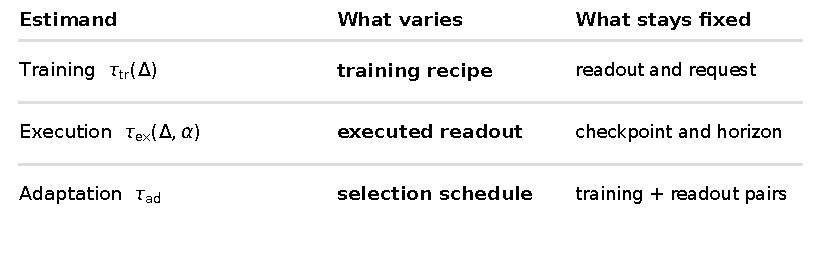
\includegraphics[width=\linewidth]{figures/estimand_taxonomy.pdf}
\caption{Three comparison targets. Training-effect contrasts vary the training recipe; execution-effect contrasts vary the executed readout at a shared checkpoint; adaptation-effect contrasts vary the per-decision selection schedule. Other factors must be matched to isolate each target.}
\label{fig:app:estimands}
\end{figure}

% ==== BRIEF Table (tab:app:estimands) =====================================
% [中] 定位：以表格形式钉死三个 estimand 的对比双方与所隔离的因素。
% 主张：其余两个因素按构造相同，这决定了每个 estimand 的含义。
% TAU-AD-96: three readings become four readings
% 证据：τ_tr、τ_ex、τ_ad 三行；τ_ad 标注 defined here, read four times without an informative result。
% 手法/边界：定义表不是结果表；τ_ad 未测量，不得读作适应收益的证据。
% [EN] Role: pins down each estimand's two sides and the factor it isolates.
% Claim: the two remaining factors are identical by construction; that fixes the meaning.
% Evidence: rows tau_tr, tau_ex, tau_ad; tau_ad is "defined here, read four times without an informative result".
% Craft/Boundaries: a definition table, not a results table; no adaptation benefit implied.
% ==== /BRIEF ==============================================================
\begin{table}[t]
\centering
\caption{The three estimands. ``Varies'' names the factor that differs between the two sides of a contrast. The remaining two factors are identical by construction, which is what fixes the estimand's meaning.}
\label{tab:app:estimands}
\small
\begin{tabular}{@{}p{2.9cm}p{4.6cm}p{4.2cm}@{}}
\toprule
Estimand & Contrast (tested vs.\ reference) & Varies / isolates \\
\midrule
Training effect $\tau_{\mathrm{tr}}(\Delta)$ & hybrid-trained model vs.\ independently trained pure-continuous model, both executing $(\Delta, \mathrm{continuous})$ & training recipe, isolating what symbol-supervised training does to the carrier \\
\addlinespace
Symbolic-execution effect $\tau_{\mathrm{ex}}(\Delta, \alpha)$ & fixed $(\Delta, \alpha)$ with $\alpha \in \{\mathrm{micro}, \mathrm{macro}\}$ vs.\ $(\Delta, \mathrm{continuous})$, inside one hybrid checkpoint & executed readout, isolating what executing a symbolic readout contributes at a fixed checkpoint \\
\addlinespace
% TAU-AD-FIX: unmeasured -> read three times without an informative result
% TAU-AD-96: three readings become four readings
Adaptation effect $\tau_{\mathrm{ad}}$ & per-decision selection policy vs.\ fixed-pair controls, within an arm at matched training & selection schedule, isolating the value of adapting granularity per decision; defined here \\
\bottomrule
\end{tabular}
\end{table}

% ==== BRIEF APP Estimands ¶2 (definitions) ================================
% [中] 定位：把三个 estimand 写成正式定义，后文引用 τ 时以此为准。
% 主张：每个 estimand 只变动一个因素，其余两个按构造固定。
% 证据：τ_tr 变训练配方、τ_ex 变执行 readout、τ_ad 变选择日程，各自列出保持相同的因素。
% 手法/边界：平铺定义、不下结论；适应效应在本文未测量。
% [EN] Role: states the three estimands formally; later uses of tau refer here.
% Claim: each estimand varies exactly one factor and holds the other two fixed by construction.
% Evidence: tau_tr varies recipe, tau_ex the executed readout, tau_ad the selection schedule.
% TAU-AD-96: three readings become four readings
% Craft/Boundaries: flat definitions, no verdict; the adaptation effect is read four times here, none informative.
% ==== /BRIEF ==============================================================
Each estimand varies exactly one factor and holds the other two fixed by construction. The \emph{training effect} $\tau_{\mathrm{tr}}(\Delta)$ varies the training recipe, comparing a model trained with symbol-supervised readouts (the hybrid arm) against an independently trained pure-continuous model, both executing the fixed continuous pair $(\Delta, \mathrm{continuous})$. The \emph{symbolic-execution effect} $\tau_{\mathrm{ex}}(\Delta, \alpha)$ varies the executed readout, comparing a fixed symbolic readout $(\Delta, \alpha)$ against the fixed continuous readout at the same $\Delta$, inside one hybrid checkpoint. The \emph{adaptation effect} $\tau_{\mathrm{ad}}$ varies the selection schedule, comparing a per-decision selection policy against fixed-pair controls within an arm at matched training. In each contrast the remaining factors are identical: readout and selection policy for $\tau_{\mathrm{tr}}$, trained model and selection policy for $\tau_{\mathrm{ex}}$, checkpoints and readouts for $\tau_{\mathrm{ad}}$.

% ==== BRIEF APP G ¶ (classification rule) =================================
% [中] 定位：分类的执行规则；全文模型比较、App E 小节首句与两次估计量切换都靠它归类。
% 主张：任一对比按两侧唯一不同的因素归入唯一估计量；τ_ad 有定义、未测量。
% 证据：三条判别规则；few-shot 减 zero-shot 的 exposure 对比标为估计量外的条件对比；两次切换：
%   配对 carrier MSE 增益、CLEVRER 递归位置 MSE。
% 手法/边界：先规则后推论；τ_ad 未测，controller 未进闭环；条件不合并；proxy 仅 heuristic。
% [EN] Role: the taxonomy's operating rule; every comparison and both switches use it.
% TAU-AD-96: three readings become four readings
% Claim: a contrast belongs to the one estimand fixed by what differs; τ_ad has four executed readings, none informative.
% Evidence: three one-factor rules; the few-shot minus zero-shot exposure contrast sits outside
%   the three; switches to paired carrier MSE and CLEVRER position MSE.
% Craft/Boundaries: no τ_ad, no closed loop; conditions unpooled; proxy heuristic.
% ==== /BRIEF ==============================================================
% TAU-AD-FIX: unmeasured -> three reported contrasts, none informative
% TAU-AD-96: add fourth reported contrast, #96
Classification is mechanical. For any contrast, examine what differs between its two sides: the training recipe alone gives a training effect, the readout at a shared checkpoint gives a symbolic-execution effect, and the selection schedule at shared checkpoints gives an adaptation effect. Under this rule, every model-comparison claim in the paper attaches to exactly one estimand: Table~\ref{tab:res:rollout} reports the training effect of symbol-supervised training at fixed requests and the symbolic-execution effect at a fixed horizon inside one hybrid checkpoint, and Section~\ref{sec:res} scores the request at one fixed checkpoint. The taxonomy extends beyond this program: any evaluation with a carrier, supervised readouts, and a selection policy can classify its contrasts the same way.

\section{Implementation Details}
\label{sec:app:impl}

\textbf{Encoder and carrier.} The 13 features of each slot are its presence probability, kind index and kind confidence, center position, velocity from the prior frame, expected-kind probability, and availability flags. The parser was trained once, on all 3,000 training lineages, and none of the calibration lineages was used for fitting the dynamics.

\textbf{Predictor.} The horizon features are $\phi(\Delta)=[\sin(\Delta\omega_j),\cos(\Delta\omega_j)]_{j=0}^{7}$ with $\omega_j=10000^{-j/8}$, the description embedding is $e_\alpha\in\mathbb{R}^{128}$, and the code is $c(r)\in\mathbb{R}^{128}$. Each $\mathrm{MLP}_\ell$ is a two-layer SiLU block, and $\gamma_\ell,\beta_\ell$ are one zero-initialized linear map of $c$ per block. The launch $a\in\mathbb{R}^5$ holds the normalized drag release, hold and tap times, and a constant. The micro head symmetrizes contact and keeps support directed; both are gated by the presence of both slots and by the head's availability output. The adapters are bias-free linear maps $650\to384$ (micro) and $4\to384$ (macro). The hybrid has 1,837,690 parameters. Counting linear layers only, one call costs 1,432,448 multiply-accumulates under $\textsf{cont}$, 1,795,456 under $\textsf{micro}$ and 1,464,704 under $\textsf{macro}$, independent of $\Delta$; the policy adds 32,128.

\textbf{Training.} Each model trains for 9,000 updates of batch 64 with AdamW (learning rate $10^{-4}$, weight decay $10^{-4}$, gradient clip 1.0), and the last update is kept, with no best-validation selection. The symbolic loss uses positive weight 5 on the predicate logits plus a cross-entropy on the availability output, with unavailable frames masked.

\textbf{Request policy.} Each of the two rounds runs 1,800 updates of batch 128 (learning rate $10^{-3}$) on the first window of each shot from 603 policy lineages. The compute term of Equation~\ref{eq:objective} counts linear multiply-accumulates of the predictor and the policy, and its normalizer is the predictor-only continuous transition at $\Delta=15$. The hybrid policy (width 128) has 32,265 parameters.

\textbf{Baseline.} The baseline width is the width in $\{384,392,\dots,512\}$ whose parameter count is nearest the hybrid's, with ties to the smaller width; its policy width, 131, is chosen by the same rule against the hybrid policy (32,229 parameters). Parameter counts are matched.

\textbf{Training used for the compute comparison.} The compute comparison of Section~\ref{sec:introduction} uses an earlier training of both models by the same recipe on the 2,400 base-corpus lineages alone, with 600 policy lineages and the same three seeds.

% ==== BRIEF APP I (sec:app:repro) =========================================
% [中] 定位：从结果转向仪器：结论要能被别人重算才算数。
% 主张：每个发表的表都能用一条 --validate 命令重算。
% 证据：表 19，每个 artifact 家族一行。
% 手法/边界：标题平铺；validate 不重训、不开新评测。
% [EN] Role: from results to the instrument: a finding counts only if others can recompute it.
% Claim: every published table recomputes with one --validate command.
% Evidence: Table 19, one row per artifact family.
% Craft/Boundaries: plain heading; validation never retrains and opens no new evaluation.
% ==== /BRIEF =============================================================
\section{Reproduction Commands}
\label{sec:app:repro}

% ==== BRIEF APP I ¶1 (environment) ========================================
% [中] 定位：给出表 19 每一行都依赖的环境与源版本约定。
% 主张：每个 --validate 从保留 artifact 重算发表表格，必须 exit 0，从不重训。
% 证据：env.sh；env@254720f（#74、#77）；0a0dd73 加 ac2a4e1、8399f57、9e369c4（#79、#80）；三个
% flag 为 false。
% 手法/边界：flag 与 commit 逐字；这是不变量，不是结果。
% [EN] Role: fixes the environment and revisions every Table 19 command assumes.
% Claim: each --validate recomputes published tables from retained artifacts and must exit 0.
% Evidence: env@254720f (#74, #77); 0a0dd73 plus ac2a4e1, 8399f57, 9e369c4 (#79, #80);
% fresh_evaluation_opened=false and two more false flags.
% Craft/Boundaries: flags and commits verbatim; an invariant, not a result; nothing retrains.
% ==== /BRIEF =============================================================
Activate the environment before running any command: \texttt{conda activate novphy \&\& source env.sh}, where \texttt{env.sh} puts the repository root on \texttt{PYTHONPATH}. All commands below run from the NovPhy repository root. The recorded source revisions are \texttt{env@254720f} for the \#74 and \#77 records and commits \texttt{0a0dd73} plus \texttt{ac2a4e1}, \texttt{8399f57}, and \texttt{9e369c4} for the \#79 line. Each \texttt{-{}-validate} mode recomputes the published tables from the retained artifacts and must exit 0. The validators never retrain a model. The external-baseline validator was verified on both cpu and cuda. Table~\ref{tab:app:repro} lists one row per artifact family.

{\small
\setlength{\LTleft}{0pt}
\setlength{\LTright}{0pt}
% ==== BRIEF Table 19 (tab:app:repro) ======================================
% [中] 定位：每个 artifact 家族一行：root 与精确命令。
% 主张：#15 到 #95 的每个家族都有一个 root 与一条 validate 命令。
% 证据：#15 至 #95 各行，如 scripts.run_launch_power_probe（#94）。
% 手法/边界：逐字；列入只说明可重算，不说明主张成立。
% [EN] Role: one row per artifact family: its root and its exact command.
% Claim: every family from #15 to #95 has one root and one validate command.
% Evidence: rows #15 to #95, e.g. scripts.run_launch_power_followup (#95).
% Craft/Boundaries: verbatim; a row certifies recomputation, not a claim (see Table 14).
% ==== /BRIEF =============================================================
\begin{longtable}{@{}p{0.22\textwidth}p{0.30\textwidth}p{0.45\textwidth}@{}}
\caption{Exact validation commands per artifact family, with artifact roots relative to the NovPhy repository root.}
\label{tab:app:repro}\\
\toprule
Artifact family & Root(s) & Command \\
\midrule
\endfirsthead
\multicolumn{3}{@{}l@{}}{\footnotesize\emph{Table \ref{tab:app:repro} (continued)}}\\
\toprule
Artifact family & Root(s) & Command \\
\midrule
\endhead
\midrule\multicolumn{3}{@{}r@{}}{\footnotesize\emph{continued overleaf}}\\
\endfoot
\bottomrule
\endlastfoot
\#74 matched systems & \texttt{.local-\allowbreak artifacts/\allowbreak issue-\allowbreak 74-\allowbreak matched-\allowbreak dynamics-\allowbreak v1/\allowbreak } & \texttt{python -u -m scripts.run\_\allowbreak issue\_74\_matched\_dynamics --validate} \\
\#77 N1 campaign & \texttt{.local-\allowbreak artifacts/\allowbreak issue-\allowbreak 77-\allowbreak n1-\allowbreak v1/\allowbreak } & \texttt{python scripts/\allowbreak run\_issue\_77\_n1.py -\allowbreak -\allowbreak validate} \\
\#77 N1 training and diagnostic & \texttt{.local-\allowbreak artifacts/\allowbreak issue-\allowbreak 77-\allowbreak n1-\allowbreak dynamics-\allowbreak v1/\allowbreak }, \texttt{.local-\allowbreak artifacts/\allowbreak issue-\allowbreak 77-\allowbreak n1-\allowbreak diagnostic-\allowbreak v1/\allowbreak } & \texttt{python -u -m scripts.run\_\allowbreak issue\_77\_n1\_diagnostic --validate} \\
\#79 CLEVRER boundary replication & \texttt{.local-\allowbreak artifacts/\allowbreak issue-\allowbreak 79-\allowbreak clevrer-\allowbreak boundary-\allowbreak v1/\allowbreak } & \texttt{python -u -m scripts.run\_\allowbreak clevrer\_boundary\_replication --validate} \\
\#84 third family & \texttt{.local-\allowbreak artifacts/\allowbreak issue-\allowbreak 84-\allowbreak third-\allowbreak family-\allowbreak v1/\allowbreak } & \texttt{python -u -m scripts.run\_\allowbreak third\_family\_boundary\_replication --validate} \\
\#92 lookahead control & \texttt{.local-\allowbreak artifacts/\allowbreak issue-\allowbreak 92-\allowbreak lookahead-\allowbreak control-\allowbreak v1/\allowbreak } & \texttt{python -u -m scripts.run\_\allowbreak lookahead\_control --validate} \\
\#96 within-checkpoint \texttt{tau\_ad} & \texttt{.local-\allowbreak artifacts/\allowbreak issue-\allowbreak 96-\allowbreak tau-\allowbreak ad-\allowbreak within-\allowbreak checkpoint-\allowbreak v1/\allowbreak } & \texttt{python -u -m scripts.run\_\allowbreak tau\_ad\_within\_checkpoint --validate} \\ % TAU-AD-96: register exact reproducibility validation command
\end{longtable}
}

% ==== BRIEF APP I ¶2 (what validators recompute) ==========================
% [中] 定位：说明各 validator 重算什么，把可复现落成可检查的动作。
% 主张：validator 从保留 ledger 与记录重算，不做新推断。
% 证据：coverage.json 重算；CLEVRER 命令 exit 0；reactive pilot-gate 判定重算，exit 0。
% 手法/边界：exit 0 证明与记录一致，不证明主张为真。
% [EN] Role: says what each validator recomputes, so reproducibility is a checkable act.
% Claim: validators recompute from retained ledgers and records, without new inference.
% Evidence: coverage.json re-derived; CLEVRER command exits 0; pilot-gate verdict recomputed.
% Craft/Boundaries: exit 0 shows agreement with the records, not the truth of a claim.
% ==== /BRIEF =============================================================
The evaluation validators recompute every published table without new inference. The CLEVRER module records its own exact validation command in its module documentation, \texttt{python -u -m scripts.run\_\allowbreak clevrer\_boundary\_replication --validate}, which recomputes every published table and exits 0.

% ==== BRIEF APP I ¶3 (closed-loop invariants + release) ===================
% [中] 定位：交代 closed-loop 测量的执行不变量与发布边界。
% 主张：每个 runner 绑定冻结 plan.json，未完成单元记为 typed failure。
% 证据：#87、#89、#90、四个 #92、#93--#95 runner；caps 86,400 s / 10,800 s GPU / 4 workers；
% 4,187 paths 到 2b4d897。
% 手法/边界：caps 是上限不是性能；typed failure 留在分母。
% [EN] Role: states the execution invariants and the release boundary of the closed-loop runs.
% Claim: each runner binds a frozen plan.json; incomplete units become typed failures.
% Evidence: #87, #89, #90, four #92 runners, #93 to #95; caps 86,400 s wall, 10,800 s GPU, 4
% workers; 4,187 paths through 2b4d897.
% Craft/Boundaries: caps are limits, not performance; state the excluded ~15 GB per pool.
% ==== /BRIEF =============================================================
The kept runners bind a frozen \texttt{plan.json} with sha256-pinned inputs, write per-cell markers and receipts to a resumable ledger, and record every unit that does not complete as a typed failure. The small-artifact subset of every root in Table~\ref{tab:app:repro} (plans, summaries, comparisons, findings, records, receipts, and ledgers) is version-controlled through commit \texttt{2b4d897}, and the \#96 root through \texttt{0e7f921c}. Frames and native chunks, about 15\,GB per pool, are excluded. % TAU-AD-96: list published within checkpoint root

% ==== BRIEF APP J (sec:app:audit) =========================================
% [中] 定位：最后一道检查：每个读数都能指回产生它的文件。
% 主张：本文打印的每个数字在表 20 中都有 artifact 路径。
% 证据：表 20。
% 手法/边界：标题平铺；审计证明出处，不证明读法。
% [EN] Role: the last check: every reading points back to the file that produced it.
% Claim: every printed number has an artifact path in Table 20.
% Evidence: Table 20.
% Craft/Boundaries: plain heading; provenance, not interpretation.
% ==== /BRIEF =============================================================
\section{Number-to-Artifact Audit}
\label{sec:app:audit}

% #91-WP5 2026-09-23: built fresh from the tex itself by harvesting every trailing artifact comment
% (grep of `%` comments containing .local-artifacts/ or data/issue-) and every printed number of the
% main text, figure captions, and Appendices A-G. Spot-verified against the artifacts during the build:
% issue-92-selection-validity-v1/findings.md (sections 1-6), issue-92-cross-pool-audit-v1/{findings.md,
% summary.json} (37 of 42 = 26 few-shot + 11 zero-shot at ordinal 12; 5 success states per condition;
% few-shot paired +0.0067 [-0.0202, +0.0368]), issue-89-oracle-completion-v1/findings.md,
% issue-87-closed-loop-oracle-v1/plan.json (caps). One defect found and fixed in synthesis.tex and
% introduction.tex: the constant-ordinal-12 rate was printed as "about 20% of cross-split cells against
% 2.12%", but the artifact rate is 3 of 15 STATES against a 0.0212 CELL rate.
% ==== BRIEF APP J ¶1 (how to read Table 20) ===============================
% [中] 定位：告诉读者表 20 怎么读。
% 主张：表 20 把每个打印的数字映射到持有它的 artifact。
% 证据：按来源分组；路径相对 NovPhy 仓库根；root 用表 19 验证。
% 手法/边界：索引约定，不是结果；不改任何数字或舍入。
% [EN] Role: tells the reader how to use Table 20.
% Claim: Table 20 maps every printed number to the artifact that holds it.
% Evidence: rows grouped by source; paths from the repository root; roots checked by Table 19.
% Craft/Boundaries: an index convention, not a result; no number or rounding changes.
% ==== /BRIEF =============================================================
Table~\ref{tab:app:audit} maps every number printed in this paper to the artifact that holds it. Rows group numbers by source. Paths are relative to the NovPhy repository root, and each root validates with the command of Table~\ref{tab:app:repro}.

{\footnotesize
\setlength{\tabcolsep}{3pt}
% ==== BRIEF Table 20 (tab:app:audit) ======================================
% [中] 定位：全文数字总账，分 closed-loop、proxy、heuristic、protocol 四组。
% 主张：每个主张的打印值、artifact 路径与 ticket 在同一行。
% 证据：如 0/108 对 0.0780（#92）；0.1299 对 0.50 floor（#82）；13/612 与 29/612 分列。
% 手法/边界：值逐字；42/1,224 只是合计计数，不是 pooled 估计；0/72 与 support 行同读。
% [EN] Role: the ledger of every printed number, in four groups by source.
% Claim: each claim's printed values, artifact path and ticket share one row.
% Evidence: e.g. 0/108 vs 0.0780 (#92); 0.1299 vs the 0.50 floor (#82); 13/612 and 29/612
% apart.
% Craft/Boundaries: verbatim; 42/1,224 is a combined count, not pooled; read 0/72 with support.
% ==== /BRIEF =============================================================
\begin{longtable}{@{}p{0.17\textwidth}p{0.37\textwidth}p{0.36\textwidth}p{0.07\textwidth}@{}}
\caption{Number-to-artifact audit. ``Value as printed'' lists every number the paper prints for the claim, in the paper's rounding.}\label{tab:app:audit}\\
\toprule
Claim & Value as printed & Artifact path & Ticket \\
\midrule
\endfirsthead
\toprule
Claim & Value as printed & Artifact path & Ticket \\
\midrule
\endhead
\bottomrule
\endfoot
Table~\ref{tab:res:rollout} (rollout error at the last endpoint) & Recursive position MSE, three-seed mean. NovPhy, 225 frames: baseline $(1,5,15,\textsf{cont}) = 2224$, $0.281$, $0.0370$; hybrid $3141$, $0.200$, $0.0296$, plus $(15,\textsf{micro}) = 0.0313$ and $(15,\textsf{macro}) = 0.0397$. CLEVRER, 120 frames: baseline $13.5$, $0.0471$, $0.0116$; hybrid $2.98$, $0.0444$, $0.0170$, plus $(15,\textsf{micro}) = 0.0190$. Physion-Dominoes, 120 frames: baseline $182.6$, $0.0176$, $0.00114$; hybrid $167.4$, $0.0156$, $0.00128$, plus $(15,\textsf{micro}) = 0.00199$ & \nolinkurl{.local-artifacts/issue-77-n1-diagnostic-v1/summary.json}, \nolinkurl{.local-artifacts/issue-79-clevrer-boundary-v1/summary.json}, \nolinkurl{.local-artifacts/issue-84-third-family-v1/summary.json} (\texttt{per\_seed} curves \texttt{position\_mse} for \texttt{continuous\_h1/h5/h15}, \texttt{hybrid\_continuous\_h1/h5/h15}, \texttt{hybrid\_micro\_h15}, \texttt{hybrid\_macro\_h15}) & \#77, \#79, \#84 \\
Figure~\ref{fig:teaser} (real cascade, imagined requests, recursive error curves) & Start, video frames 80/120 and final video frame 554 map to carrier frames $0,80,120,553.38$ (native steps $30000,34000,36000,57669$, origin $30000$, stride $50$); the final photo is the engine-window endpoint, not the imagined endpoint $600$; the request trace comes from a decision-only imagined rollout (candidate 6: modal $1$-continuous, $29/94$ queries); F(5,macro) rank among nine in launch-angle, offset, drag-grid and launch-power order $1,1,9,4$; $J-F^{*}$ AUC differences $+.0595$, $+.0037$, $+.0700$, $+.0273$ & \nolinkurl{data/issue-87-closed-loop-oracle/manifest.json} (state/ordinal frame pointers); \nolinkurl{.local-artifacts/issue-87-closed-loop-oracle-v1/attempts/oracle--issue-77-n1-001-a00--a06/shot-1/observation-trace/observation_trace_manifest.json} (frame\_records fixed\_step); \nolinkurl{.local-artifacts/issue-92-lookahead-control-v1/records/decision--hybrid-adaptive-e600--seed20260908--issue-77-n1-001-a00.json} (decision.horizon\_trace["6"]); \nolinkurl{.local-artifacts/issue-96-tau-ad-within-checkpoint-v1/comparisons.csv} & \#87, \#92, \#96 \\
Section~\ref{sec:exp:fixed} and Figure~\ref{fig:res:grid} (per-set request ranking) & Ordering AUC per set: $(5,\textsf{macro})$ $0.63$ (angle) and $0.59$ (offset) and $0.40$ (drag grid, last of nine), $(1,\textsf{macro})$ $0.51$ (drag grid) and $0.53$ (launch power); best-minus-worst spread $0.44$--$0.51$; $r^\dagger$ trails the set's best request by $0.03$--$0.13$ & \nolinkurl{figures/build_results_grid.py} over \nolinkurl{.local-artifacts/issue-96-tau-ad-within-checkpoint-v1/comparisons.csv} (\texttt{auc\_F-*}, \texttt{spread}) & \#96 \\
Section~\ref{sec:exp:selection} (policy against the transferred fixed request) & $J-r^{\dagger}$: $+0.060$ (angle sweep), $+0.004$ (offset sweep), $+0.070$ (drag grid), $+0.027$ (launch power) & \nolinkurl{.local-artifacts/issue-96-tau-ad-within-checkpoint-v1/comparisons.csv} (\texttt{inventory\_J-F*}) & \#96 \\
Section~\ref{sec:exp:selection} (compute) & Ranking regret $0.350$ (hybrid adaptive) against $0.367$ (horizon-only adaptive); $118.7$M against $356.0$M linear MACs per candidate and state; $1.0$\,s against $2.0$\,s per state; $80$ against $189$ predictor calls per candidate and state & \nolinkurl{.local-artifacts/issue-74-matched-dynamics-v1/readiness.json} & \#74 \\
Section~\ref{sec:exp:qual} (request schedules) & 12 candidates receive eight schedules; the successful launch a6 is ranked sixth of 12 by the policy, last by $(1,\textsf{macro})$ and first by $(5,\textsf{macro})$; 2{,}634 imagined rollouts; $77\%$ of level--seed pairs differ between candidates; $\Delta=5$ share $2\%\to16\%$; $\textsf{macro}$ share $59\%\to83\%$ & \nolinkurl{.local-artifacts/issue-96-tau-ad-within-checkpoint-v1/records/} (per-cell \texttt{decision.schedules}), aggregated and plotted by \nolinkurl{figures/build_qualitative_requests.py} & \#96 \\
Ranker architecture & depth-3 predictor, 236-dimensional carrier; 1{,}837{,}690 (hybrid) and 1{,}862{,}396 (continuous) parameters; 9{,}000 updates, batch 64; 2{,}409 fitting lineages & \nolinkurl{.local-artifacts/issue-77-n1-dynamics-v1/plan.json} (\texttt{contract.config}, \texttt{training}, parameter-count block) & \#77 \\
\end{longtable}
}

% 2026-09-25 (owner directive): the Reproducibility and Ethics statements move out of the main
% body (per the ICLR example in manuscript/style_example: no such statements in the main text).
% They live here as the closing appendix sections; the main text ends with Section 8, then
% references. Both were \section* pre-reference blocks before this move (discussion.tex).
% ==== BRIEF APP K (Reproducibility Statement) =============================
% [中] 定位：收尾声明之一，从正文移入附录末尾。
% 主张：closed-loop 测量可从保留记录重算。
% 证据：指向 sec:mth:protocol、sec:app:protocol、sec:app:repro、两张表。
% 手法/边界：标题平铺；不新增事实。
% [EN] Role: the first closing statement, moved from the body to the appendix end.
% Claim: the closed-loop measurement recomputes from retained records.
% Evidence: pointers to the protocol, Appendices A and I, the registry and the audit.
% Craft/Boundaries: plain heading; no new fact.
% ==== /BRIEF =============================================================
\section{Reproducibility Statement}

Section~\ref{sec:mth:protocol} defines the evaluation protocol, Appendix~\ref{sec:app:protocol} records its mechanics and typed-failure taxonomy, and Appendix~\ref{sec:app:repro} gives the validation command for every cited artifact root. The records behind Sections~\ref{sec:res} and~\ref{sec:disc} recompute from retained artifacts: the \#74 matched-systems runner, the \#77 N1 training and diagnostic runner, the CLEVRER replication runner, the third-family runner, the \#92 lookahead-control runner, and the \#96 within-checkpoint runner, each rerun as \texttt{python -u -m scripts.\{runner\} -{}-validate}, with module names and commands listed in Table~\ref{tab:app:repro}. Each run binds a frozen \texttt{plan.json} with sha256-pinned inputs and writes per-cell markers and receipts to a resumable ledger, and every unit that does not complete ends as a typed failure of a recorded kind. The small-artifact subset of every cited root (plans, summaries, comparisons, findings, records, receipts, and ledgers) is version-controlled through commit \texttt{2b4d897}, and the within-checkpoint root through \texttt{0e7f921c}. Frames and native chunks (about 15\,GB per pool) are excluded. Table~\ref{tab:app:audit} maps every printed number to its artifact path. % TAU-AD-96: add thirteenth reproducibility validation runner

% ==== BRIEF APP L (Ethics Statement) ======================================
% [中] 定位：收尾声明之二：界定研究对象的范围。
% 主张：本工作只涉及模拟环境。
% 证据：下段所列的 NovPhy 场景与 CLEVRER 标注发布。
% 手法/边界：标题平铺。
% [EN] Role: the second closing statement: it bounds what the work touches.
% Claim: the work involves simulated environments only.
% Evidence: the NovPhy scenarios and CLEVRER annotation release named below.
% Craft/Boundaries: plain heading.
% ==== /BRIEF =============================================================
\section{Ethics Statement}
% ==== BRIEF APP L ¶1 (ethics) =============================================
% [中] 定位：说明本工作用什么、不触及什么；全文在此结束。
% 主张：只用模拟物理环境；无人类受试者、个人数据或已部署系统。
% 证据：NovPhy 场景；CLEVRER 标注发布，CC0 许可。
% 手法/边界：照实短写；NovPhy 是已发表 benchmark，不是本文新数据。
% [EN] Role: states what the work uses and what it does not touch; the paper ends here.
% Claim: simulated physics only; no human subjects, personal data or deployed systems.
% Evidence: NovPhy scenarios; the CLEVRER annotation release under CC0.
% Craft/Boundaries: short and literal; NovPhy is a published benchmark, not new data.
% ==== /BRIEF =============================================================
This work uses simulated physics environments only: NovPhy scenarios and the CLEVRER annotation release, which is distributed under a CC0 license. It involves no human subjects, personal data, or deployed systems.


